
\RequirePackage{currfile} 
\documentclass{beamer}



%%%%%%%%%%%%%% PACKAGES %%%%%%%%%%%%%%%%%%%%%
\usepackage{textpos}   
\usepackage{graphicx} % Allows including images
\usepackage{booktabs} % Allows the use of \toprule, \midrule and \bottomrule in tables
\usepackage{biblatex} % Allows for \cite 
\usepackage[utf8]{inputenc}
\usepackage{tikz} \usetikzlibrary{calc, arrows.meta, intersections, patterns, positioning, shapes.misc, fadings, through,decorations.pathreplacing}
\usepackage{array} % To pause columns
\usepackage[usenames,dvipsnames]{xcolor}
\usepackage{colortbl}
\usepackage{multicol}
\usepackage{multirow}
\usepackage{caption}
%\usepackage{block} %blocks for statements
\usepackage{comment}
\usepackage[absolute,overlay]{textpos}
\usepackage{forest}
\forestset{qtree/.style={for tree={parent anchor=south, 
           child anchor=north,align=center,inner sep=0pt}}}


% Custom block colors for better appearance
\setbeamercolor{block title}{bg=blue!20,fg=black}
\setbeamercolor{block body}{bg=blue!10,fg=black}
\setbeamertemplate{blocks}[rounded][shadow=true]


\definecolor{ColorOne}{named}{MidnightBlue}
\definecolor{ColorTwo}{named}{Dandelion}
\definecolor{ColorThree}{named}{Plum}

\tikzstyle{descript} = [text = black,align=center, minimum height=1.8cm, align=center, outer sep=0pt,font = \footnotesize]
\tikzstyle{activity} =[align=center,outer sep=1pt]

%% Change the bg color to adjust your transition slide background color!
\newenvironment{transitionframe}{
  \setbeamercolor{background canvas}{bg=White}
  \begin{frame}}{
    \end{frame}
}

%%%%%%%%%%%%%% COMMANDS %%%%%%%%%%%%%%%%%%%%%
\newcommand{\progressbar}{%
\pgfmathsetmacro{\theta}{360/\inserttotalframenumber*\insertframenumber}
\begin{tikzpicture}[scale=0.025]
\fill[blue] (0,0) circle (9);
\fill[green] (0,0) -- (9,0) arc (0:-\theta:9);
\fill[white] (0,0) circle (5);
\node at (0,0) {\insertframenumber};
\end{tikzpicture}
}

%%% TIKZ STUFF
\tikzset{   
        every picture/.style={remember picture,baseline},
        every node/.style={anchor=base,align=center,outer sep=1.5pt},
        every path/.style={thick},
        }
\newcommand\marktopleft[1]{%
    \tikz[overlay,remember picture] 
        \node (marker-#1-a) at (-.3em,.3em) {};%
}
\newcommand\markbottomright[2]{%
    \tikz[overlay,remember picture] 
        \node (marker-#1-b) at (0em,0em) {};%
}
\tikzstyle{every picture}+=[remember picture] 
\tikzstyle{mybox} =[draw=black, very thick, rectangle, inner sep=10pt, inner ysep=20pt]
\tikzstyle{fancytitle} =[draw=black,fill=red, text=white]
%%%% END TIKZ STUFF

%%% COLOR COLUMN (did not make it work...)
\newcolumntype{G}{>{\centering\columncolor{gray!20!white}}p{0.2\textwidth}}
\newcolumntype{C}{>{\centering\arraybackslash}p{0.2\textwidth}}
%%% END COLOR COLUMN


\AtBeginSection[]{
  \begin{frame}
  \vfill
  \centering
  \begin{beamercolorbox}[sep=8pt,center,shadow=true,rounded=true]{title}
    \usebeamerfont{title}\insertsectionhead\par%
  \end{beamercolorbox}
  \vfill
  \end{frame}
}

%%%%%%%%%%%%%%% SETTINGS %%%%%%%%%%%%%%%%%%%%%%%
\mode<presentation> {
%\usetheme{Warsaw}
%\usetheme{Frankfurt}
%\usetheme{Madrid}
\usetheme{default}
%\usecolortheme{whale}
\usecolortheme{default}
\usefonttheme{professionalfonts}
}

%To call references
%\bibliographystyle{../aea.bst}
%\bibliography{references}

%%%%%%%%%%%%%%%%%%%%%%%%%%%%%%%%%%
%FOR LINKS
\definecolor{darkblue}{rgb}{0.0, 0.0, 0.65}
\definecolor{darkgreen}{rgb}{0.0, 0.65, 0.0}
\hypersetup{
	citecolor=blue,
	colorlinks=true,
	linkcolor=blue,
	filecolor=magenta,
	urlcolor=magenta
}
%%%%%%%%%%%%%%%%%%%%%%%%%%%%%%%%%%


\setbeamertemplate{navigation symbols}{} 


%Title
\title[]{When the Household Becomes the School: Sibling Effects on Parental Attention and Educational Outcomes During School Closures}
%\subtitle[]{DLP Writing Seminar}

\author[Francisco Pardo] % (optional, for multiple authors)
{Francisco Pardo - fpardo@utexas.edu \inst{1}}
 
\institute[UT] % (optional)
{
  \inst{1}%
  University of Texas at Austin
  %\and
  %\inst{2}%
   % ...
}

\date{\today}
 

 
 
%------------------------------------------------------------
%The next block of commands puts the table of contents at the 
%beginning of each section and highlights the current section:
%Commented because presentations are short, we don't need that. 
\begin{comment}
\AtBeginSection[]
{
  \begin{frame}
    \frametitle{Table of Contents}
    \tableofcontents[currentsection]
  \end{frame}
}
\end{comment}
%------------------------------------------------------------

\begin{document}


\frame{\titlepage}


\begin{frame}
    \label{update_scott}
    \frametitle{Motivation}
    \begin{enumerate}
        \item Persistent learning losses from Covid-19 across the world, especially in more vulnerable populations. %\textcolor{blue}{cite}
        \item With school closures and kids at home, parents spent more time in childcare and education.
        \item Unexpected changes in family size have negative spillovers. \textcolor{blue}{Black et al (2010)}
        \item No evidence of the role of family size in places with significant school closures.
        

        \begin{block}{Research Question}
Do students with siblings experience larger learning losses through the pandemic compared to only children? Is this because of dilution of parental resources?
\end{block}
    \end{enumerate}
\end{frame}

\begin{frame}
    \label{update_scott}
    \frametitle{Contribution to literature}
    \begin{enumerate}
        %\item \textbf{Covid Learning Loss} \\
        %\item \textbf{Universal Pre-K}: Is there a sibling spillover effect in this space due to released time? I see new literature like Jackson et al (2025), Humphries et al (2025) mostly on increased labor/earnings.
        %\item \textbf{Health Shocks}: 
        %\begin{itemize}
        %    \item Siblings with disabilities: Black et a
        %\end{itemize}
        %\item \textbf{Parental Investment} \\
        %\item \textbf{Quanity-Quality} \\
        %\item \textbf{Universal PreK:} \\
        %$\uparrow$ labor and earnings. Benefits $>>>$ Costs. \\
        %\small \textcolor{gray}{Jackson, Turner, Bastian (2025), Humphries et al (2025)}

    \end{enumerate}
\end{frame}


% ========================================
% DATA
% ========================================
\begin{frame}
    \frametitle{Data}

    \begin{itemize}
        \item School progression (approval and GPA per grade-year)
        \item Standardized test scores in 2nd, 4th, 6th, 8th grade in some years.
        \item Family, student, teachers and principals surveys:
        \begin{itemize}
            \item Parental involvement in children's education
            \item Socioeconomic Status
            \item Aspirations for higher education: parents (2nd and 4th grade) and students (8th grade)
            %\item Gender beliefs: "Boys are better at Math than girls"
            %\item Parental involvement: my parents ask me about my grades, I talk to my parents about what I read, why they chose school, gender beliefs, overall knowledge about school/child, etc
            %\item studying habits, beliefs, etc
            %\item Specifically related to siblings: ``Read out loud to my siblings''.
        \end{itemize}
        \item Identify siblings through parent's anonymized ID.
    \end{itemize}
\end{frame}

% ========================================
% DATA
% ========================================
\begin{frame}
    \frametitle{Trends in data}
    \begin{columns}[T]
        \begin{column}{0.48\textwidth}
            \centering
            \textbf{\% of A's in Mathematics}
            \vspace{0.2cm}
            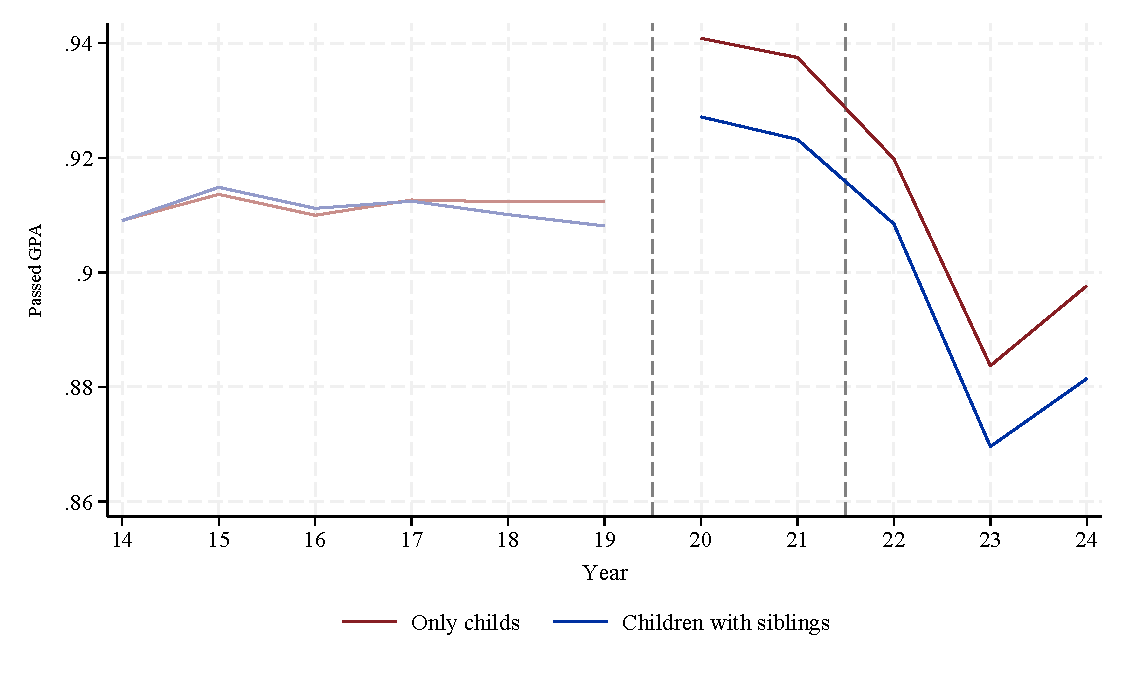
\includegraphics[width=\textwidth]{./FIGURES/Descriptive/raw_total_elm_pass_math_siblings.pdf}
        \end{column}
        \begin{column}{0.48\textwidth}
            \centering
            \textbf{Standardized GPA in Mathematics}
            \vspace{0.2cm}
            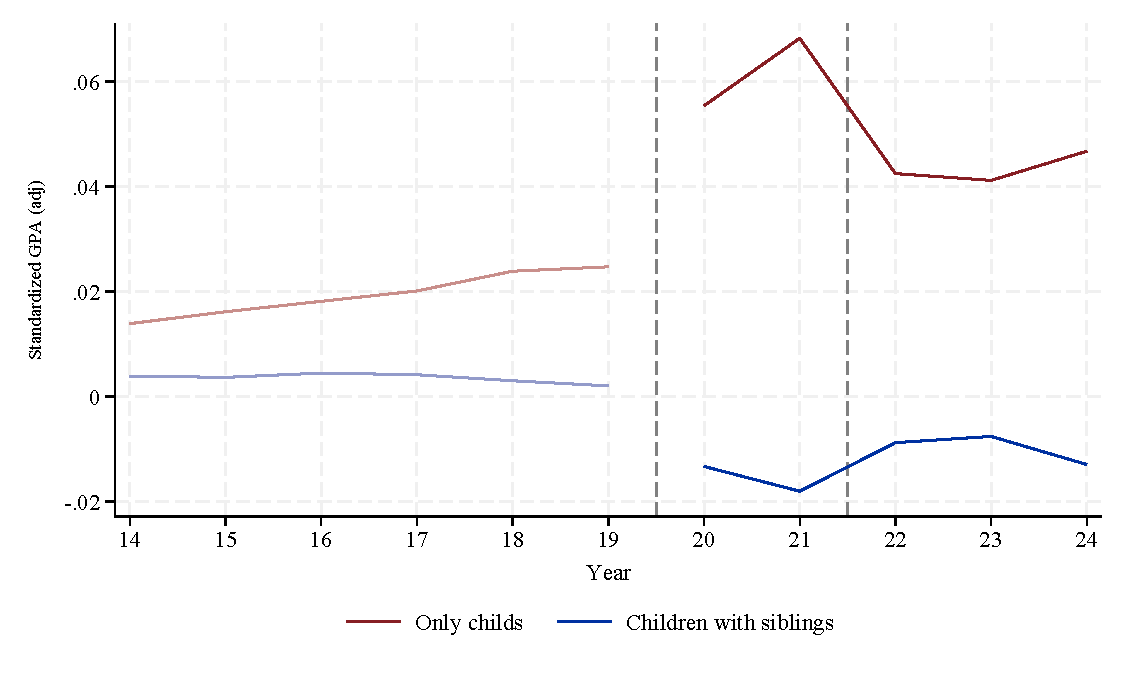
\includegraphics[width=\textwidth]{./FIGURES/Descriptive/raw_total_elm_std_gpa_m_adj_siblings.pdf}
        \end{column}
    \end{columns}
    
    
\end{frame}


% ========================================
% EMPIRICAL STRATEGY
% ========================================
\begin{frame}
    \frametitle{Identification Strategy}
    
    \begin{block}{Identification Strategy}
    Differential changes between only children and children with siblings before and after the pandemic.
    \end{block}
    
    \textbf{Difference-in-Differences Specification:}
    \small
    \begin{align}
    Y_{ist} &= \alpha + \delta_1 \text{Post}_{it} + \delta_2 \text{HasSiblings}_{i} \nonumber  \\
    &\quad + \boldsymbol{\beta} (\text{Post}_{it} \times \text{HasSiblings}_{i}) \nonumber \\
    &\quad + \mathbf{X}_{ist}'\gamma + \lambda_s + \mu_t + \varepsilon_{ist}
    \end{align}
    
    \vspace{0.1cm}
    
    \textbf{Event Study Specification:}
    \begin{align}
    Y_{ist} &= \alpha + \sum_{k=-5}^{-2} \delta_k (\mathbb{I}[t = 2020+k] \times \text{HasSiblings}_{i}) \nonumber \\
    & \quad + \sum_{k=0}^{4} \beta_k (\mathbb{I}[t = 2020 + k] \times \text{HasSiblings}_{i}) \nonumber \\
    & \quad + \mathbf{X}_{ist}'\gamma + \text{HasSiblings}_{i} + \lambda_s + \mu_t + \varepsilon_{ist}
    \end{align}
    \normalsize
    
    %where $\tau_d$ is the treatment date for district $d$, and we normalize $\beta_{-1} = \delta_{-1} = 0$.
    
\end{frame}


% ========================================
% RESULTS
% ========================================

\begin{frame}
    \frametitle{Event Study - Mathematics GPA}
        {\resizebox{0.9\textwidth}{!}{
       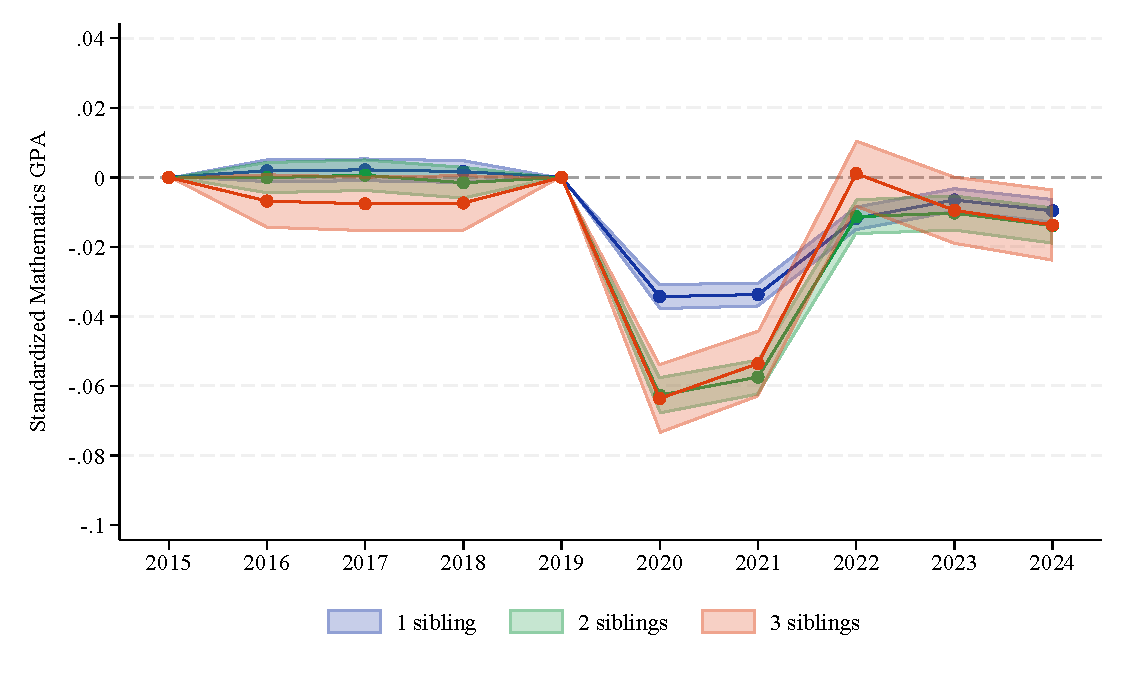
\includegraphics{./FIGURES/Event Study/covid_event_bysibs_all_all_std_gpa_m_adj_Tsiblings_Soldest_4.pdf}
      }
    }
\end{frame}

\begin{frame}
    \frametitle{TWFE results}
        {\resizebox{0.9\textwidth}{!}{
       %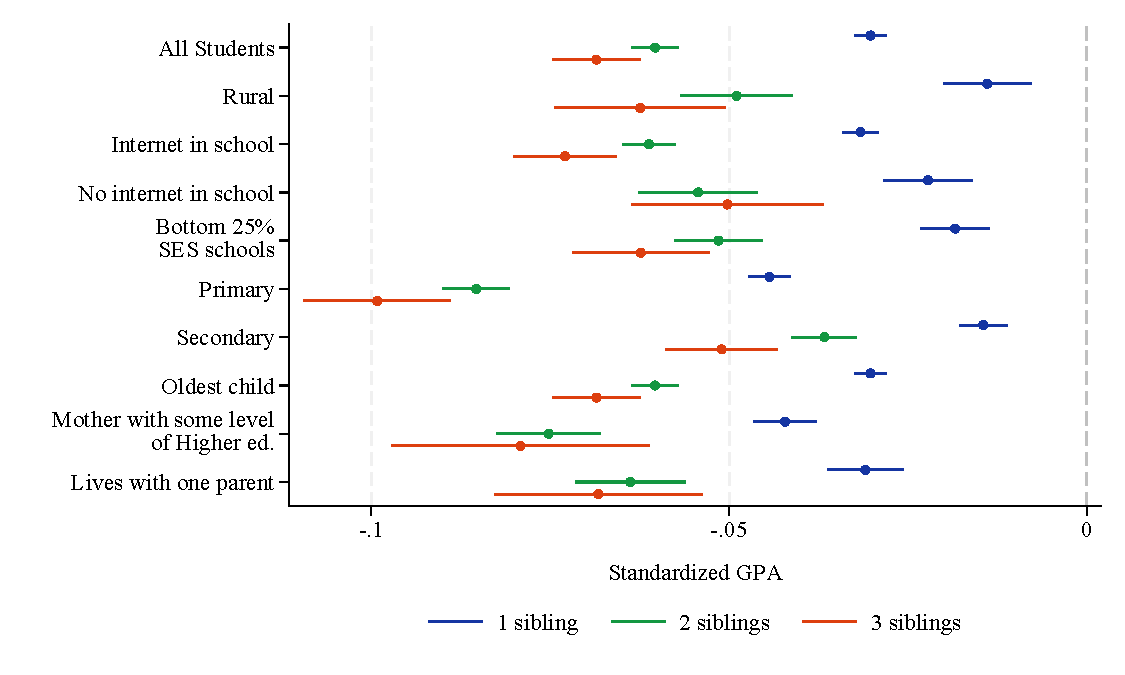
\includegraphics{./FIGURES/TWFE/covid_twfe_summ_bysibs_all_20-21_gpa_m_adj_Tsiblings_Soldest_4.pdf}
       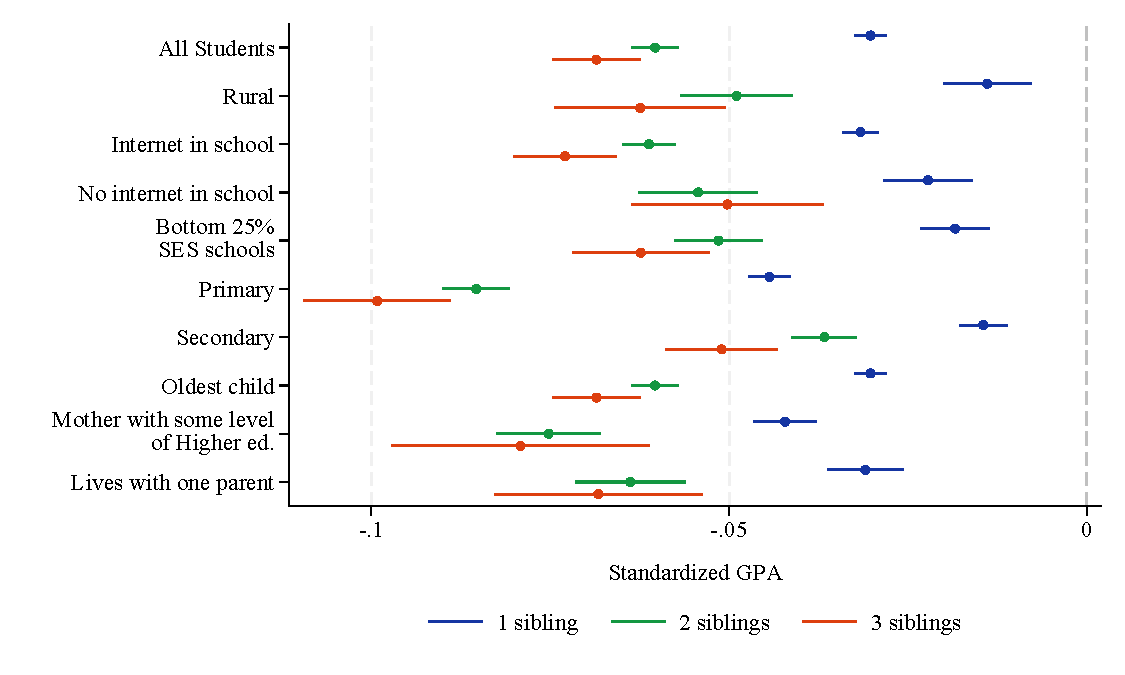
\includegraphics{./FIGURES/TWFE/covid_twfe_summ_bysibs_all_20-21_gpa_m_adj_Tsiblings_Soldest_4.pdf}
      }
    }
\end{frame}


\begin{frame}
\frametitle{TWFE - Standardized Exams}
       \centering
       \resizebox{0.7\textwidth}{!}%
{
\makeatother
\begin{tabular}{lcccc}
\toprule
\cmidrule(lr){2-5}
& \multicolumn{4}{c}{TWFE} \\
\cmidrule(lr){2-5}
& 1-3 siblings & 1 sibling & 2 siblings & 3 siblings  \\
\cmidrule(lr){2-2} \cmidrule(lr){3-3} \cmidrule(lr){4-4} \cmidrule(lr){5-5}
& (1) & (2) & (3) & (4) \\
\bottomrule
&  &  & &  \\
&  &  & &  \\
\multicolumn{5}{l}{Panel A: GPA } \\
Mathematics         &      -0.099***&      -0.011   &      -0.036***&      -0.059***\\
                    &     (0.009)   &     (0.009)   &     (0.011)   &     (0.015)   \\
                    &               &               &               &               \\ 
&  &  & &  \\
Reading             &      -0.099***&      -0.010   &      -0.031***&      -0.034** \\
                    &     (0.009)   &     (0.009)   &     (0.010)   &     (0.015)   \\
                    &               &               &               &               \\
Observations        &     326,669   &     280,846   &     225,840   &     180,218   \\
 
&  &  & &  \\
\multicolumn{5}{l}{Panel B: Standardized Exams } \\
Mathematics         &      -0.034***&      -0.017** &      -0.044***&      -0.071***\\
                    &     (0.006)   &     (0.007)   &     (0.008)   &     (0.011)   \\
                    &               &               &               &               \\ 
&  &  & &  \\
Reading             &      -0.013** &       0.002   &      -0.022***&      -0.046***\\
                    &     (0.006)   &     (0.006)   &     (0.008)   &     (0.011)   \\
                    &               &               &               &               \\
Observations        &     409,690   &     282,769   &     227,486   &     181,466   \\
 

\bottomrule
\end{tabular}
}

\end{frame}

\begin{comment}
\begin{frame}
    \frametitle{Main Results}
    
\end{frame}

\begin{frame}
    \frametitle{Main Results}
    
\end{frame}
\end{comment}
% ========================================
% MECHANISMS
% ========================================
\begin{frame}
    \frametitle{Potential Mechanisms}
    \begin{itemize}
        \item Birth Order
        \item Scarce material resources
        \item Sibling disruption
        \item Parental dilution
        \item Income Shocks
    \end{itemize} 
\end{frame}

\begin{frame}
    \frametitle{Birth Order}
        {\resizebox{0.9\textwidth}{!}{
        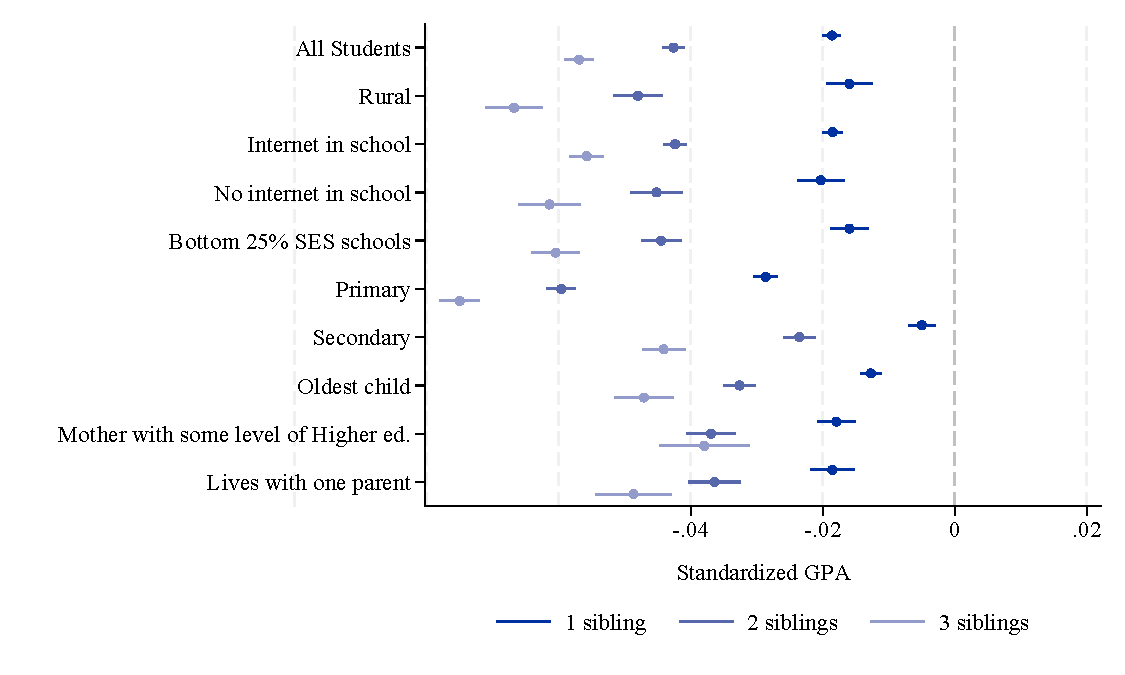
\includegraphics{./FIGURES/TWFE/covid_twfe_sibs_summ_all_all_gpa_m_adj_siblings_4.pdf}
      }
    }    
\end{frame}

\begin{frame}
    \frametitle{Scarce material resources: Socio Economic Status}
       \centering
       \resizebox{0.7\textwidth}{!}{
\makeatother
\begin{tabular}{lcccc}
\toprule
\cmidrule(lr){2-5}
& \multicolumn{4}{c}{TWFE} \\
\cmidrule(lr){2-5}
& 1-3 siblings & 1 sibling & 2 siblings & 3 siblings  \\
\cmidrule(lr){2-2} \cmidrule(lr){3-3} \cmidrule(lr){4-4} \cmidrule(lr){5-5}
& (1) & (2) & (3) & (4) \\
\bottomrule
&  &  & &  \\
&  &  & &  \\

\multicolumn{5}{l}{Panel B: Low SES Households (Q1)} \\
Mathematics         &      -0.028***&      -0.009   &      -0.036***&      -0.061***\\
                    &     (0.005)   &     (0.006)   &     (0.006)   &     (0.008)   \\
 
&  &  & &  \\
Reading             &      -0.022***&      -0.010   &      -0.029***&      -0.044***\\
                    &     (0.005)   &     (0.006)   &     (0.007)   &     (0.008)   \\
                    &               &               &               &               \\
Observations        &     643,621   &     398,084   &     358,488   &     290,244   \\
 
&  &  & &  \\
\multicolumn{5}{l}{Panel C: High SES Households (Q4)} \\
Mathematics         &      -0.035***&      -0.029***&      -0.051***&      -0.072***\\
                    &     (0.006)   &     (0.007)   &     (0.009)   &     (0.019)   \\
 
&  &  & &  \\
Reading             &      -0.039***&      -0.032***&      -0.068***&      -0.010   \\
                    &     (0.006)   &     (0.007)   &     (0.010)   &     (0.019)   \\
                    &               &               &               &               \\
Observations        &     385,616   &     318,633   &     230,174   &     186,296   \\
 

\bottomrule
\end{tabular}
}

\end{frame}


\begin{frame}
    \frametitle{Scarce material resources: PC and Internet}
       \centering
       \resizebox{0.7\textwidth}{!}{
\makeatother
\begin{tabular}{lcccc}
\toprule
\cmidrule(lr){2-5}
& \multicolumn{4}{c}{TWFE} \\
\cmidrule(lr){2-5}
& 1-3 siblings & 1 sibling & 2 siblings & 3 siblings  \\
\cmidrule(lr){2-2} \cmidrule(lr){3-3} \cmidrule(lr){4-4} \cmidrule(lr){5-5}
& (1) & (2) & (3) & (4) \\
\bottomrule
&  &  & &  \\
\multicolumn{5}{l}{Panel D: Households with no PC or Internet} \\
Mathematics         &      -0.037***&      -0.024***&      -0.067***&      -0.089***\\
                    &     (0.005)   &     (0.005)   &     (0.006)   &     (0.010)   \\
 
&  &  & &  \\
Reading             &      -0.036***&      -0.025***&      -0.063***&      -0.083***\\
                    &     (0.005)   &     (0.005)   &     (0.006)   &     (0.010)   \\
                    &               &               &               &               \\
Observations        &     766,875   &     566,628   &     447,252   &     356,075   \\
 
&  &  & &  \\
\multicolumn{5}{l}{Panel E: Households with both PC and Internet} \\
Mathematics         &      -0.043***&      -0.024***&      -0.051***&      -0.080***\\
                    &     (0.005)   &     (0.005)   &     (0.006)   &     (0.008)   \\
 
&  &  & &  \\
Reading             &      -0.035***&      -0.018***&      -0.049***&      -0.054***\\
                    &     (0.005)   &     (0.005)   &     (0.006)   &     (0.008)   \\
                    &               &               &               &               \\
Observations        &     793,797   &     552,557   &     452,886   &     360,214   \\
 

\bottomrule
\end{tabular}
}

\end{frame}



\begin{frame}
    \frametitle{Sibling disruption}
        {\resizebox{0.9\textwidth}{!}{
        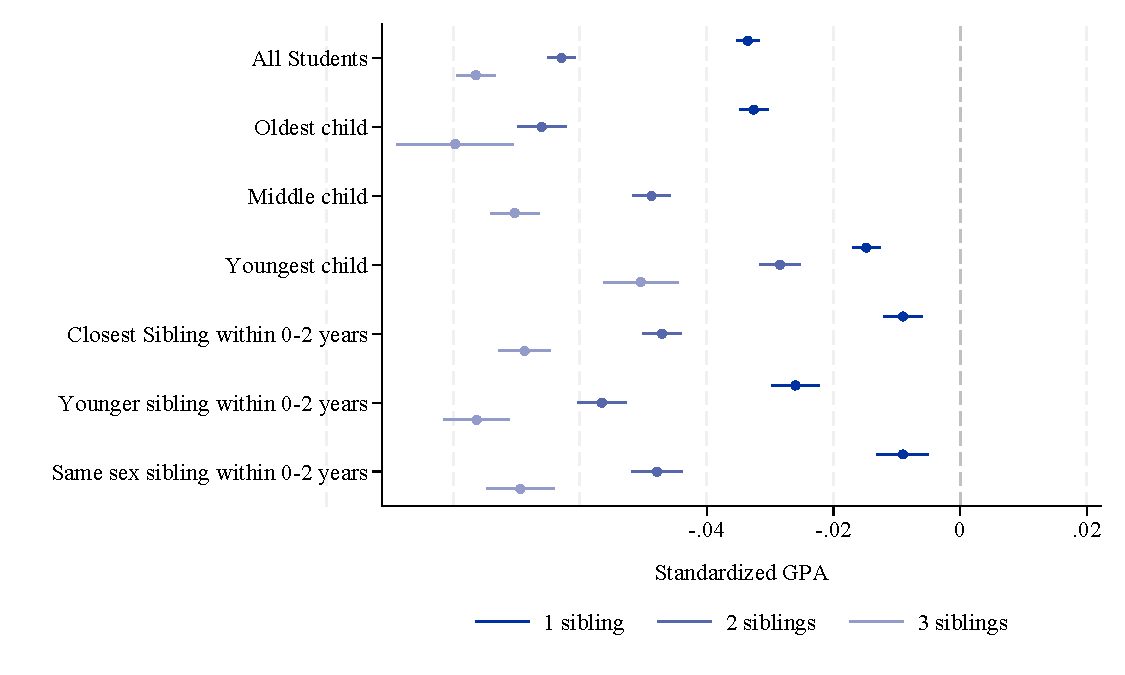
\includegraphics{./FIGURES/TWFE/covid_twfe_sibs_C_elm_all_gpa_m_adj_4.pdf}
      }
    }

\end{frame}

\begin{frame}
    \frametitle{Parental dilution}
        {\resizebox{0.9\textwidth}{!}{
        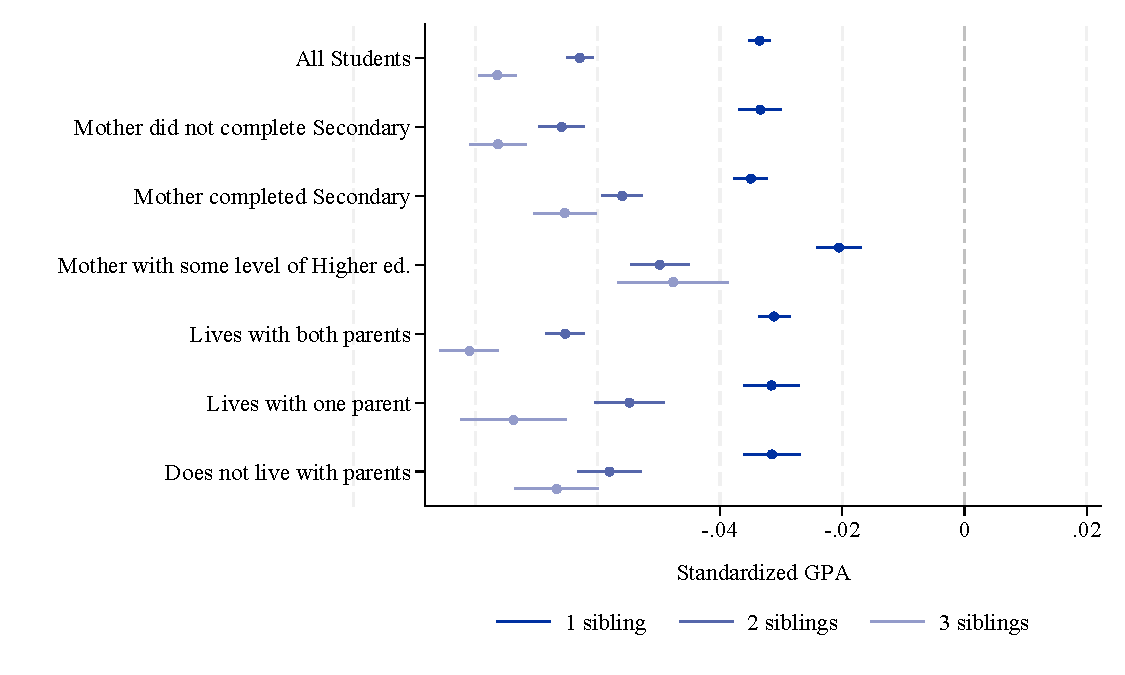
\includegraphics{./FIGURES/TWFE/covid_twfe_sibs_D_elm_all_gpa_m_adj_4.pdf}
      }
    }

\end{frame}

\begin{frame}
    \frametitle{Parental dilution - Increased childcare}
       \begin{itemize}
            \item We use effects of delayed schooling (more childcare) outside of Covid to have a sense of how parents react to this.
            \item Mixed results in literature (US and Denmark) although not until younger starts school.
        \end{itemize}
\end{frame}      

\begin{frame}
    \frametitle{Effects of delaying younger School Entry (GPA of older)}
    \makeatletter
\@ifclassloaded{beamer}{%
       \centering
       \resizebox{0.6\textwidth}{!}%
}{%
       \begin{table}[!tbp]\centering\def\sym#1{\ifmmode^{#1}\else\(^{#1}\)\fi}
       \centering
       \caption{Effects of younger sibling delaying school on older sibling standardized exams - 1 - m - a -  - 365}
       \label{tab:rd_summ_1_m_a_365}
       \resizebox{0.95\textwidth}{!}%
}
{
\makeatother
\resizebox{\textwidth}{!}{
\begin{tabular}{lccc}
\toprule
\cmidrule(lr){2-4}
& \multicolumn{3}{c}{Standardized GPA} \\
\cmidrule(lr){2-4}
& Pre-Covid & Covid & Post-Covid  \\
& 2018-2019 & 2020-2021 & 2022-2023  \\
\cmidrule(lr){2-2} \cmidrule(lr){3-3} \cmidrule(lr){4-4}
& (1) & (2) & (3)  \\
\bottomrule
&  &  &   \\
\multirow{2}{*}{\shortstack[l]{Younger sibling born after \\ school-entry cutoff}}&      -0.023***&      -0.001   &      -0.023***\\
                    &     (0.007)   &     (0.007)   &     (0.006)   \\
Local Linear        &         Yes   &         Yes   &         Yes   \\
                    &               &               &               \\
Observations        &     358,861   &     354,044   &     447,536   \\
Counterfactual mean &       0.058   &       0.020   &       0.050   \\
Bandwidth           &         365   &         365   &         365   \\
 

\bottomrule
\end{tabular}
}
\@ifclassloaded{beamer}{%
}{%
       \end{table}
}

\end{frame}

\begin{frame}
    \frametitle{Effects of delaying younger School Entry (Scores and investment)}
\makeatletter
     \centering
       \resizebox{0.95\textwidth}{!}%
{
\makeatother
\begin{tabular}{lccccc}
\toprule
& \multicolumn{2}{c}{Pre-Covid}  & \multicolumn{3}{c}{Post-Covid} \\
& \multicolumn{2}{c}{2018-2019}  & \multicolumn{3}{c}{2022-2024}  \\
\cmidrule(lr){2-3} \cmidrule(lr){4-6}
& Mathematics & Reading & Mathematics & Reading & Parental Investment  \\
& (1) & (2) & (3) & (4) & (5) \\
\bottomrule
&  &  &  & &  \\
\multirow{2}{*}{\shortstack[l]{Younger sibling born after \\ school-entry cutoff}}&      -0.025*  &      -0.023*  &      -0.009   &      -0.012   &      -0.035***\\
                    &     (0.014)   &     (0.012)   &     (0.013)   &     (0.010)   &     (0.013)   \\
Local Linear        &         Yes   &         Yes   &         Yes   &         Yes   &         Yes   \\
                    &               &               &               &               &               \\
Observations        &      86,605   &      86,602   &     104,983   &     105,064   &     101,766   \\
Counterfactual mean &      -0.105   &      -0.083   &       0.194   &       0.288   &      -0.004   \\
Bandwidth           &         365   &         365   &         365   &         365   &         365   \\
 

\bottomrule
\end{tabular}
}


\end{frame}

\begin{frame}
    \frametitle{Income Shocks}
     

\end{frame}

\begin{frame}
    \frametitle{Other potential strategies}
        \begin{itemize}
            \item Twin births: exogenous change in family size.
            \begin{itemize}
                \item Results are not significant
                \item $\approx$ 1,000 observations per grade-year of first-born with twin siblings
                \item This measures the effect of 3rd relative to 2nd child, not the effect of 2nd relative to 1st.
            \end{itemize}
            \item Same sex as instrument
            \begin{itemize}
                \item Has more power
                \item `expected change' in family size but couple with our shock may become `unexpected'
            \end{itemize}
            
        \end{itemize}
     

\end{frame}


\begin{frame}
    \frametitle{Effect of family size on GPA: Using Twin IV}
    \begin{table}[h]
\centering
\caption{Effect of Family Size on GPA}
\label{tab:twfe_twins}
\resizebox{0.95\textwidth}{!}{%
\begin{tabular}{lHccccHcccc}
\hline
& \multicolumn{5}{c}{Pre-Covid} & \multicolumn{5}{c}{Covid (2020-2021)} \\
\cmidrule(lr){2-6} \cmidrule(lr){7-11}
& OLS & OLS & First & Second & N & OLS & OLS & First & Second & N \\
& (no controls) & (controls) & Stage & Stage & & (no controls) & (controls) & Stage & Stage & \\
\hline
& & & & & & & & & & \\
Instrument: first two children same sex & & & 0.050* & & 3,300,349 & & & 0.047* & & 2,809,126 \\
\quad (Sample: first and second children in families & & & (0.001) & & & & & (0.001) & & \\
\quad with two or more births) & & & & & & & & & & \\
Number of children in family & $-0.081$* & $-0.070$* & & 0.063* & & $-0.119$* & $-0.101$* & & $-0.031$ & \\
& (0.001) & (0.001) & & (0.022) & & (0.001) & (0.001) & & (0.025) & \\
Instrument: twin at second birth & & & 0.813* & & 1,589,159 & & & 0.855* & & 1,240,864 \\
\quad (Sample: First child in families with two or more & & & (0.006) & & & & & (0.006) & & \\
\quad births) & & & & & & & & & & \\
Number of children in family & $-0.090$* & $-0.056$* & & 0.012 & & $-0.125$* & $-0.085$* & & 0.009 & \\
& (0.001) & (0.001) & & (0.012) & & (0.002) & (0.002) & & (0.013) & \\
& & & & & & & & & & \\
%Instrument: twin at third birth & & & 0.819* & & 1,195,717 & & & 0.866* & & 841,770 \\
%\quad (Sample: first and second children in families & & & (0.006) & & & & & (0.006) & & \\
%\quad with three or more births) & & & & & & & & & & \\
%Number of children in family & $-0.104$* & $-0.090$* & & $-0.020$ & & $-0.118$* & $-0.101$* & & $-0.019$ & \\
%& (0.002) & (0.002) & & (0.013) & & (0.002) & (0.002) & & (0.014) & \\
%& & & & & & & & & & \\
\hline
\end{tabular}%
}
\end{table}
\end{frame}

% ========================================
% EXTERNAL VALIDITY
% ========================================
\section{External Validity}

    \begin{frame}
            \frametitle{Looking at PISA data)}
        \begin{itemize}
            \item International examination to 15 year olds
            \item 81 countries (37 OECD and 44 non-OECD).
            \item In 2009, 2012 and 2022, I am able to identify only-child and sibling sample.
            \item I estimate the gap in achievement between both for each of these years.
        \end{itemize}
    \end{frame}

\begin{frame}
    \frametitle{Learning gaps in Mathematics by year}
    
    \begin{figure}
        \centering
        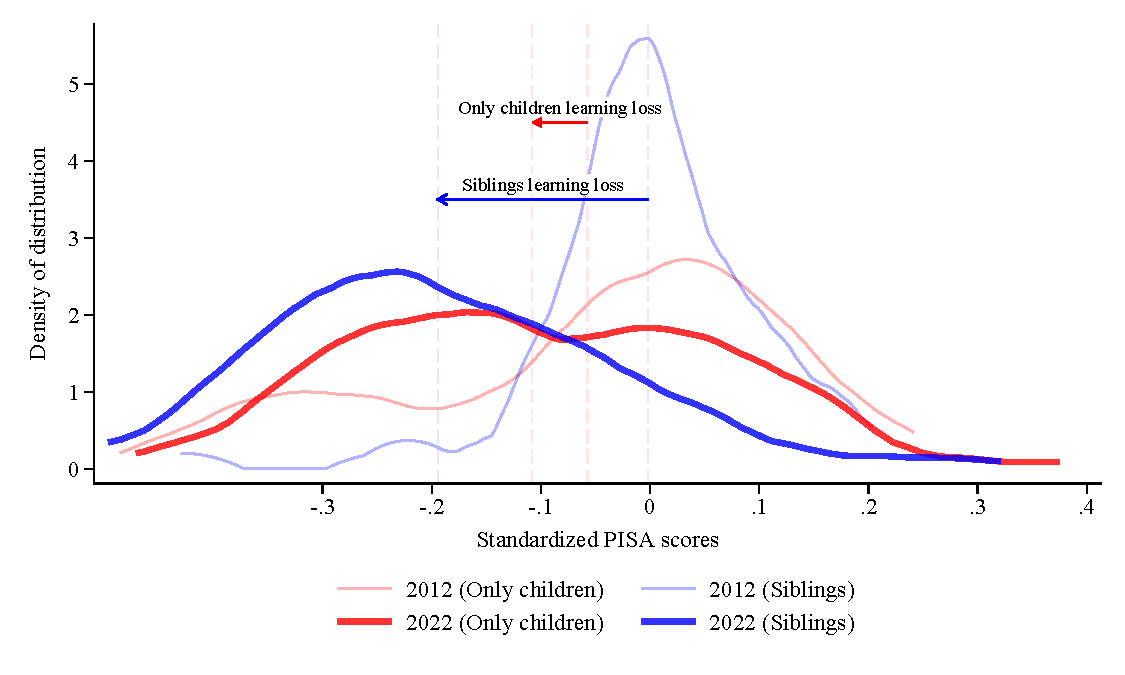
\includegraphics[width=0.9\textwidth]{./FIGURES/Descriptive/PISA_distribution_2012_2022_PV4MATH.pdf}
        \caption{Learning gaps in Mathematics by year}
        \label{fig:1a}
    \end{figure}
    
\end{frame}

\begin{frame}
    \frametitle{Change in learning gaps by duration of school closure}
    
    \begin{figure}
        \centering
        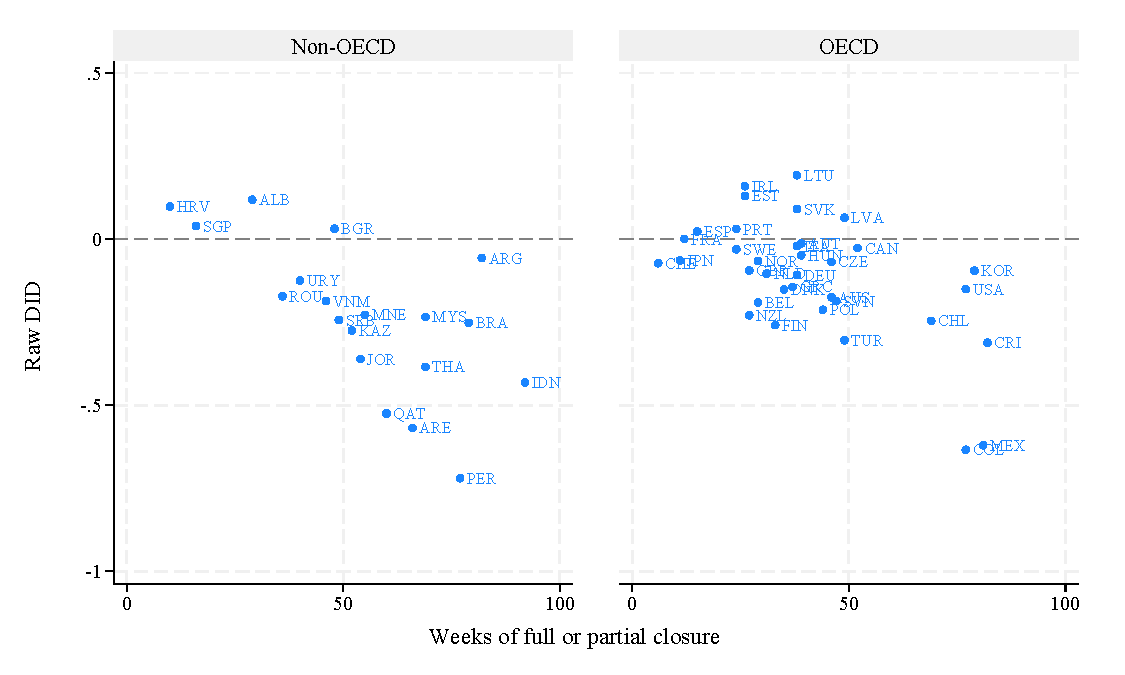
\includegraphics[width=0.9\textwidth]{./FIGURES/Descriptive/PISA_raw_DID_PV4MATH_not_fully_open.pdf}
        \caption{Change in learning gaps by duration of school closure for OECD and Non-OECD countries}
        \label{fig:1b}
    \end{figure}
    
\end{frame}

% ========================================
% EXTERNAL VALIDITY
% ========================================
\section{Conclusions}

\end{document}